%
\documentclass[12pt,a4paper,ngerman,twoside]{report}
%\documentclass[12pt,twoside]{report}
%
%
\usepackage[dvips]{graphics}
\graphicspath{{./Bilder/}}
\usepackage{epsfig}
\usepackage[ansinew,latin1]{inputenc} % wichtig f�r Umlaute
\usepackage{babel}
\usepackage{amssymb}
\usepackage{amsmath} % wichtig f�r die align-Umgebung in Formeln
% f�r das Einbinden von Quelltexte
\usepackage{color} 
\usepackage{titlesec} % Text�berschriften anpassen

\definecolor{middlegray}{rgb}{.6,0.6,.6}      % grau

\usepackage{listings} 
\lstset{numbers=left, numberstyle=\tiny, numbersep=5pt} 
\lstset{language=C}
\lstset{
   basicstyle=\scriptsize\ttfamily,
   keywordstyle=\bfseries\ttfamily\color{blue},
   stringstyle=\color{green}\ttfamily,
   commentstyle=\color{middlegray}\ttfamily,
   emph={square}, 
   emphstyle=\color{blue}\texttt,
   emph={[2]root,base},
   emphstyle={[2]\color{yac}\texttt},
   showstringspaces=false,
   flexiblecolumns=false,
   tabsize=2,
   numbers=left,
   numberstyle=\tiny,
   numberblanklines=false,
   stepnumber=1,
   numbersep=10pt,
   xleftmargin=15pt
 }



\usepackage{dsfont}
%
\usepackage{thesis}
	%

\begin{document}

\pagestyle{empty}   % Rueckseite des titelblattes
	%
%
%---------------------------------------------
%
%	beleg_titel.tex
%
%---------------------------------------------
	%
	%
	%	
	%
\pagestyle{empty}	% Rueckseite des titelblattes
\begin{center}
{\large
	Hochschule f�r Telekommunikation Leipzig\\[1em]
	Fakult�t Informations- und Kommunikationstechnik\\
	Institut f�r Kommunikationstechnik
}\\
\vfil
	%
{\large\bf
	Abschlussarbeit zum Erlangen des akademischen Grades\\[1ex]
	Master of Engineering
}
\end{center}

\vfil

\begin{tabbing}
% platzhalter
Themensteller:w\=\kill
	%
Thema:\>
{\large
	Empfehlungen zum Anfertigen von wissenschaftlichen Arbeiten
}\\[8em]

vorgelegt von:\>	Hans Mustermann\\[2em]
geboren am:\>			25.09.1990\\
in:\>							Finsterberg-Dodeleben\\[3em]
Themensteller:\>	Institut f�r Kommunikationstechnik, HfTL\\
							\>  Gustav-Freitag-Str. 43-45\\
							\>	04277 Leipzig\\[2em]
Erstpr�fer:\>			Prof. Dr.-Ing. habil. Lene Lehmann\\[1em]
Zweitpr�fer:\>		Dr.-Ing. Malte M�ller\\[2em]
Datum:\>					\today
\end{tabbing} % 
	%
\cleardoublepage
%
%---------------------------------------------
%
%   kurzreferat.tex
%
%---------------------------------------------
	%
% 
\chapter*{Kurzreferat}

\begin{quote}
Das Kurzreferat ist eine Art Zusammenfassung, welche die wichtigsten Informationen zur Arbeit enth�lt (Worum geht es �berhaupt? Welche wesentliche Methode wurde eingesetzt zur L�sung des Problems? Was sind die wichtigsten Ergebnisse?)

Das Schreiben von wissenschaftlichen Arbeit ist einfach, wenn man es schon zehn mal gemacht hat. Studenten, die zum ersten Mal mit dieser Aufgabe konfrontiert werden, wissen zumeist noch nicht einmal, welche Schriftart benutzt werden sollte. Diese Arbeit gibt eine allgemeine Empfehlung �ber inhaltliche und �u�erliche Gestaltung von wissenschaftlichen Arbeiten. Das Layout ist durch ein \LaTeX-Stylefile definiert. Auch wenn andere Textverarbeitungssysteme verwendet werden m�ssen, sind die Richtlinien in diesem Text zu beachten. Die Anmerkungen in dieser Arbeit helfen dem Studenten, seine praktische Arbeit in schriftlicher Form logisch und informativ zu dokumentieren.
\end{quote} % 
	%
\cleardoublepage

%---------------------------------------------
%
%	formel.tex
%
%---------------------------------------------
	%
\chapter*{Formelzeichen und Abk"urzungen}
	%
	%
%
%-------------------------------------------------------
\begin{tabbing}
	%
ABCDEF\=Erl"auterung\kill\\
	%
$\korresp$	\> Korrespondenz zwischen einem Zeitsignal und seinem Spektrum\\
$\lfloor x.y \rfloor$ \> ganzzahliger Anteil von $x.y$ \lt $x $\\
$\lceil x.y \rceil$ \> kleinster ganzzahliger Wert gr"o"ser gleich $x.y$ \lt $\left\{ \begin{array}{cl}
					x 	& , y=0\\
					x+1	& , y\neq 0
					\end{array}\right.$\\
$<\ul{a}, \ul{b}>$	\> Skalarprodukt der Vektoren $\ul{a}$ und $\ul{b}$\\
$[t_k,t_{k+1})$	\> Intervall in den Grenzen von einschlie"slich $t_k$ bis ausschlie"slich $t_{k+1}$\\
$a_n, a[n$]	\>Approximations- oder Tiefpasskoeffizient \\
$x[n]$		\>zeitdiskretes Signal, Folge von Symbolen	\\
$X(z)$		\>zeitdiskretes Signal im $\cal{Z}$-Bereich	\\
%$zs$		\>Anzahl der Zerlegungsstufen bei der dyadischen Wavelet-Transformation \\
${\mathds{Z}}$	\> Menge der ganzen Zahlen
	%
\end{tabbing}
	%
\vfil
	%
%Abkuerzungen
%-------------------------------------------------------
\begin{tabbing}
	%
ABCDEF\=Erl"auterung\kill\\
	%
AKF	\> Autokorrelationsfunktion\\
CODEC	\> enCOder/DECoder \\
CQF	\> Konjugiert-Quadratur-Filterbank (engl.: {\em conjugate quadrature filterbank}) \\
MPEG	\> Motion Picture Experts Group	\\
MSE	\> mittlerer quadratischer Fehler (engl.: {\em mean square error}) \\
MUX	\> Multiplexer \\
	%
\end{tabbing}
	%

\pagestyle{headings}
\pagenumbering{roman}
%\setcounter{page}{2}
	%
	%
\cleardoublepage
\tableofcontents
\cleardoublepage
%
\pagenumbering{arabic}
	%
	%
%\listoffigures
%\listoftables
%\cleardoublepage
	%
\renewcommand{\baselinestretch}{1.1}
\small\normalsize
%\setlength{\parskip}{0.2\baselineskip plus 0.3ex minus 0.1ex}
%

%
%-------------------------------------------------------
%
% nuetzliche Definitionen siehe thesis.sty
%
%-------------------------------------------------------
%
	%
%---------------------------------------------
%
%   einleitung.tex
%
%---------------------------------------------
	%
	%
	%
%----------------------------------------------
\chapter{Einleitung}
%----------------------------------------------
	%
{\em Die Einleitung sollte so einfach geschrieben sein, dass JEDER versteht, worum es in dieser Arbeit geht. Es ist nicht zwingend erforderlich, die Einleitung zu untergliedern.}
	%
%-------------------------------------------------------
\section{Thematischer Hintergrund}
	%
Warum wurde die Arbeit angefertigt?\\
Worum geht es hier eigentlich thematisch gesehen?\\
Was gab es schon vorher?\\
Wie ordnet sich die Arbeit in das Wissenschaftsgebiet ein?\\
	%
%-------------------------------------------------------
\section{Motivation und Zielstellung}
	%
Was soll jetzt neu untersucht werden?\\
Was erhofft man sich davon?\\
	%
%-------------------------------------------------------
\section{Gliederung der Arbeit}
	%
Was steht in den einzelnen Kapiteln geschrieben?\\
Jedes Kapitel beginnt auf einer neuen Seite!\\
Die Arbeit ist vorzugsweise mit dem Textsatzsystem \LaTeX\ zu schreiben!
	%
%----------------------------------------------

%---------------------------------------------
%
%   grundlagen.tex
%
%---------------------------------------------
	%
%----------------------------------------------
\chapter{Grundlagen}
%----------------------------------------------
	%
{\em In diesem Kapitel werden alle f{\"u}r die Arbeit erforderlichen theoretischen und praktischen Grundlagen behandelt. Im Hauptteil der Arbeit kann man sich darauf beziehen.}
	
	%
%----------------------------------------------
\section{Was ist wissenschaftliches Arbeiten?}
%----------------------------------------------
	%
	%
%----------------------------------------------
\subsection{Der Prozess des wissenschaftlichen Arbeitens}
%----------------------------------------------

Am Anfang einer wissenschaftlichen Arbeit stehen die Themasuche und die Problemdefinition. Anschlie�end erfolgt die Materialsuche und Materialauswahl. Dabei sollten Sie beachten, stets seri�se und zuverl�ssige Quellen auszuw�hlen. Beispielsweise gilt die Online-Enzyklop�die Wikipedia bei vielen Professoren als unseri�s, weshalb das Zitieren von Texten dieser Plattform in wissenschaftlichen Arbeiten nur nach R�cksprache mit dem Lehrenden zu empfehlen ist. Nach der Materialsuche und Materialauswahl erfolgt das Auswerten des Materials sowie das Verfassen einer Gliederung. Erst wenn Sie die Gliederung der wissenschaftlichen Arbeit festgelegt haben, sollten Sie mit der schriftlichen Ausarbeitung beginnen.
%Dieser Prozess zur Erstellung einer wissenschaftlichen Arbeit wird als wissenschaftliches Arbeiten verstanden. Ein Thema bzw. eine Problemstellung wird nach wissenschaftlichen Standards und Prinzipien mit wissenschaftlichen Verfahren und Techniken bearbeitet.
	%
%----------------------------------------------
\subsection{Merkmale des wissenschaftlichen Arbeitens}
%----------------------------------------------
	%
Nach Prei�ner (\cite{Prei94}) lassen sich folgende Merkmale des wissenschaftlichen Arbeitens identifizieren:
\begin{itemize}
  \item	Wissenschaftliches Arbeiten ist systematisches Arbeiten. Um eine nachvollziehbare Argumentation zu gew�hrleisten, muss die Arbeit einen klaren Aufbau besitzen, aus dem der Gang der Untersuchung hervorgeht.
  \item	Wissenschaftliches Arbeiten hei�t objektiv begr�nden. Verzichten Sie auf gef�hlsm��ige Argumentation. Jedes Ihrer Urteile muss auf nachvollziehbaren Kriterien basieren. Die Herkunft und Quelle aller wesentlichen Gedanken sind dabei stets anzugeben.
  \item	Wissenschaftliches Arbeiten ist Streben nach Allgemeing�ltigkeit. Achten Sie darauf, dass Ihre Aussagen auf mehrere F�lle �bertragbar sind. Geben Sie stets den G�ltigkeitsbereich Ihrer Erkenntnisse an.
  \item	Wissenschaftliches Arbeiten ist auch das Auseinandersetzen mit anderen Arbeiten. Ihr grundlegendes Ziel sollte sein, einen Beitrag zum wissenschaftlichen Fortschritt zu leisten. Dazu ist erforderlich, den Stand der Forschung zu dokumentieren und eigenst�ndige Schlussfolgerungen zu ziehen bzw. durch eigene Forschung darauf aufzubauen.
  \item	Wissenschaftliches Arbeiten kann auf Basis von Literaturauswertung, empirischer Analyse oder einer Kombination aus beidem erfolgen. Bei der Literaturauswertung sollten Sie auf eine ausgewogene Auswahl der Quellen achten. Ber�cksichtigen Sie unterschiedliche Lehrmeinungen und achten Sie darauf, dass eine verwendete �u�erung allgemein anerkannt ist. Bei empirischen Untersuchungen ist stets zu fragen, ob das Ergebnis repr�sentativ ist. Um eine Kritik des Erhebungs- und Auswertungsverfahren zu erm�glichen, m�ssen die Materialien auch immer einsehbar sein.
  \item	Die wesentlichen Begriffe einer wissenschaftlichen Arbeit m�ssen definiert werden. Die Bedeutung vieler Fachbegriffe ist nicht eindeutig festgelegt. Um eine einheitliche Diskussionsgrundlage zu schaffen, muss das der Arbeit zugrunde gelegte Verst�ndnis eines Begriffes gekl�rt werden.
\end{itemize}
	%
	Neben diesen Standards und Prinzipien sind beim Erstellen einer wissenschaftlichen Arbeit auch formale Anspr�che zu ber�cksichtigen. So verf�gen wissenschaftliche Arbeiten �ber einen fest vorgegebenen Aufbau, bestehend aus Titelseite, Inhaltsverzeichnis, Vorwort, Kurzreferat (Abstract), Literaturverzeichnis sowie gegebenenfalls Abbildungs-, Tabellen-, Abk�rzungs- und Symbolverzeichnis. 
	
Mit dem Bearbeiten der vorgegebenen Themenstellung und dem Verfassen einer wissenschaftlichen Arbeit erbringt der Verfasser den Nachweis, dass er in der Lage ist, eine Aufgabenstellung seiner Studienrichtung mit Hilfe wissenschaftlicher Methoden und Erkenntnisse zu beschreiben, L�sungen zu erarbeiten und diese darzustellen. Dabei steht eine systematische und strukturierte Arbeitsweise im Vordergrund, die einen eigenen sch�pferischen Anteil an der L�sungsfindung erkennen l�sst. 

Grunds�tzlich beinhaltet die ingenieurm��ige Vorgehensweise immer wiederkehrende Arbeitsschritte:
	%
	\begin{itemize}
	\item Problemanalyse, Abgrenzen der Themenstellung,
	\item Beschreibung des Standes der Technik und Einordnung des Themas durch Recherche,
	\item Pr�zisieren der Themenstellung und Beschreibung von Zielen,
	\item Erarbeiten von L�sungsans�tzen, L�sungswegen, Versuchsplanungen, Programmabl�ufe,
	\item Untergliederung in Teilaufgaben und -l�sungen sowie deren Abh�ngigkeiten,
	\item Musteraufbauten, Simulationen, Programmtests,
	\item Zusammenfassung und Wertung der Ergebnisse,
	\item Schlussfolgerungen f�r weitere Arbeiten.
	\end{itemize}
		%
Alle Darlegungen sind klar und pr�zise sowie eindeutig zu formulieren. Bilder, Tabellen und Gleichungen sind in den Text einzuarbeiten. Im Text ist darauf Bezug zu nehmen. 
Die benutzten Quellen sind im Literaturverzeichnis aufzunehmen. Im Textteil sowie in Bild- und Tabellenbeschriftungen sind die Quellenverweise anzugeben. F�r die Textdarstellung gelten die Regeln der Rechtschreibung der Sprache, in der die Arbeit verfasst wird.

Anlagen sind Texte, Bilder, Tabellen, die nicht unmittelbar zur Zielentwicklung der Arbeit beitragen, aber dennoch f�r das Verst�ndnis des Gesamtkontextes wichtig sind. Sie enthalten tiefer gehende erkl�rende Informationen �ber einen speziellen Aspekt der Arbeit, die der Autor f�r erw�hnenswert h�lt.
	%
%----------------------------------------------
\subsection{Regeln zur Sicherung guter wissenschaftlicher Praxis}
%----------------------------------------------
	%
Im Zeitalter des leichtgemachten Plagiats sind Regeln der guten wissenschaftlichen Praxis unabdingbar. An der HfTL gibt es eine entsprechende Verfahrensordnung \cite{VO08}.	
%-------------------------------------------------
\section{Layout}
%----------------------------------------------
	%
%-------------------------------------------------------
\subsection{Formatierung} 
%-------------------------------------------------------
Sowohl f�r Text als auch �berschriften sollte der Font \glqq Times New Roman\grqq\ verwendet werden. Das ist in \LaTeX\ die Standardvorgabe. Die Schriftgr��e des Textes sollte 12pt sein. Links und rechts wird ein Seitenrand von ca. 2.5 cm empfohlen. Die R�nder oben und unten ergeben sich durch einen Textspiegel von 160 mm $\times$ 240 mm. Der Zeilenabstand ist in diesem Dokument auf 1.1 gesetzt. Es ist Blocksatz zu verwenden und die automatische Silbentrennung zu aktivieren.

Abk�rzungen sind beim erstmaligen Gebrauch im Text auszuschreiben und unmittelbar dahinter ist die Abk�rzung in runden Klammern anzugeben. F�r verwendete Formelzeichen ist im Text die zugeordnete physikalische Gr��e zu benennen.
	%
%-------------------------------------------------------
\subsection{Notation} 
%-------------------------------------------------------
    %
Skalare Variables werden {\it kursiv} geschrieben, zum Beispiel, $y$, $f(x)$, $a_1$ etc. Vektoren werden durch kleine, fett gedruckte Buchstaben, wie z.B.\  $\mathbf{x}= (x_1, x_2, \dots x_N)^{\rm T}$ gekennzeichnet. Der Exponent ${\rm T}$ bedeutet \glqq transponiert\grqq , sodass $\mathbf{x}$ ein Spaltenvektor ist. Bitte beachten, dass ${\rm T}$  nicht {\it kursiv} geschrieben ist, weil es sich hier nicht um eine Variable handelt. Das Gleiche gilt f�r Indizes, welche keine laufenden Nummern sind, wie $i$ in $y_i$, sondern welche nur signalisieren, dass eine Variable sich auf etwas Bestimmtes bezieht, wie bei $\sigma^2_{\rm y}$. ${\rm y}$ ist hier keine laufende Nummer; es zeigt an, dass $\sigma^2$ die Varianz in $y$ ist. F�r Matrizen werden gro�e, fett gedruckte Buchstaben verwendet, wie $\mathbf{J}$ und $\mathbf{W}$, zum Beispiel.
	%
%-------------------------------------------------------
\subsection{Schreibstil} 
%-------------------------------------------------------
    %
	Die Abschlussarbeit ist in der Regel in deutscher Sprache zu verfassen. Festlegungen zur Ausfertigung in einer anderen Sprache bed�rfen der Best�tigung aller am Verfahren beteiligten Personen.

Beachten Sie, dass es in wissenschaftlichen Arbeiten un�blich ist, in der Ich- oder Wir-Form zu schreiben. Notfalls wird zum Umschreiben das Passiv oder \glqq man\grqq\ genutzt.

Das Substantivieren von Verben durch die Endung "`ung"' sollte vermieden werden, wenn m�glich. Oft kann man eine anderes Wort verwenden. Statt "`die Differenzierung"' k�nnte man entweder "`die Differentiation"' oder einfach "`das Differenzieren"' schreiben. Manchmal ist sogar der Sinn ein anderer, wie zum Beispiel bei "`das Bestimmen"' und "`die Bestimmung"'. Auch bezeichnet "`das Darstellen"' mehr einen Vorgang, w�hrend "`die Darstellung"' eher das Ergebnis eines Vorganges ist (ebenso: "`das Abbilden"' $\leftrightarrow$ "`die Abbildung"' oder "`das Formulieren"' $\leftrightarrow$ "`die Formulierung"'). "`das Erstellen von"' ist sprachlich besser als "`die Erstellung von"'.

Alles im Sinne von "`das Kuchen-Backen"' ist okay, aber "`die Kuchen-Backung"' wohl eher nicht.
	%
%-------------------------------------------------------
\subsection{Einbinden von Tabellen und Abbildungen}
	%
\Tabe{tab_thresholds1} zeigt ein Tabellenbeispiel.
	%
\begin{table}
\centering % Zentrieren der Tabelle
  \caption{\label{tab_thresholds1}Beispiel f�r das Einbinden von Tabellen}
\begin{tabular}{|c|c|c|c|}
  \hline
  Bereich & $Q_i$ & Bereich & $Q_i$\\
  \hline
  $\infty$ .. -T3 & -4 & T3 .. $\infty$ &4 \\
  -T3+1 .. -T2    & -3 & T2 .. T3-1     &3 \\
  -T2+1 .. -T1    & -2 & T1 .. T2-1     &2 \\
  -T1+1 .. -1     & -1 &  1 .. T1-1     &1 \\
  0               &  0 &                & \\
  \hline
\end{tabular}
\end{table}
	%
Tabellen haben �blicher Weise eine Tabellen\-�ber\-schrift, w�hrend Abbildungen eine Unterschrift haben. Das ist beispielhaft in \Abbg{fig_YUV} dargestellt.
	%
\begin{figure}%[hbt]
  \hfil 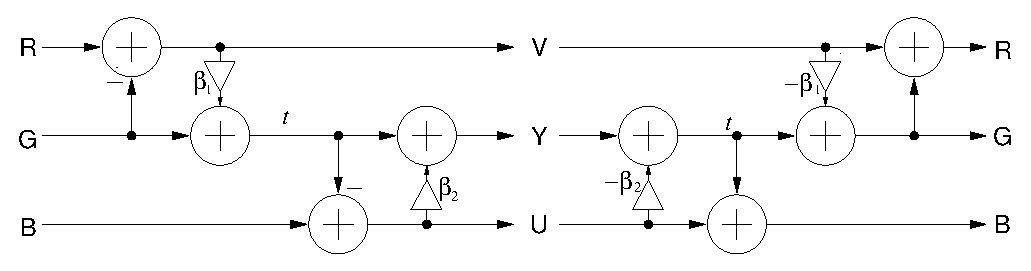
\includegraphics[scale=0.7]{./Bilder/YUV2_all.eps}
  \caption{\label{fig_YUV}Signalfluss-Beispiel f�r eine Farbraumtransformation}
\end{figure}
	%
%
%-------------------------------------------------------
\subsection{Literaturverzeichnis}
	%
Zum Referenzieren von Literatur wird ein System vorgeschlagen, dass die ersten drei Buchstaben des Nachnamens des Erstautors und die beiden letzten Ziffern des Jahres der Ver�ffentlichung enthalten \cite{Fli93}. Die Literatureintr�ge sind dann alphabetisch zu sortieren. Alternative ist auch ein Nummerieren in der Reihenfolge der Referenzierungen m�glich. Die erste Variante hat den Vorteil, dass der Leser aus der Angabe schon nach einmaligem Nachschlagen ableiten kann, um welche Literaturangabe es sich handelt.
 %
%-------------------------------------------------------
\subsection{Formelzeichenverzeichnis}
	%
Ein Formelzeichenverzeichnis (Nomenklatur) sollte angelegt werden, wenn viele Symbole verwendet werden, die einer Erl�uterung bed�rfen. Das Erstellen dieses Verzeichnis ist auch manchmal hilfreich, um Doppelbelegungen von Buchstaben (Symbolen) aufzusp�ren und auszumerzen.
	%
%-------------------------------------------------------
\subsection{Umfang der Arbeit}
	%
Der Umfang einer Abschlussarbeit sollte ohne Anhang folgende Seitenzahl nicht �ber\-schrei\-ten:
\begin{itemize}
\item Master-Arbeit: 100 Seiten,
\item Bachelor-Arbeit: 60 Seiten,
\item Studien-/Projektarbeit: 30 Seiten.
\end{itemize}
	%
	%
%-------------------------------------------------------
\subsection{Formatierungsvorlagen}
	%
Es ist empfehlenswert, f�r das Anfertigen der schriftlichen Arbeit eine geeignete Vorlage zu verwenden. Die LaTeX-Vorlage f�r dieses Dokument ist frei verf�gbar \cite{Latex}. Eine Anleitung zum Benutzen von LaTeX in Verbindung mit dem Editor TeXnicCenter findet man im Anhang \ref{app_B} dieses Dokumentes.
	%
%-------------------------------------------------------
\subsection{Kriterien zur Bewertung der Abschlussarbeit}
	%
Der Ma�stab zur Bewertung einer Abschlussarbeit h�ngt stark vom Fachgebiet ab. Die formalen Anforderungen an die schriftliche Arbeit lassen sich aber weitestgehend von den obigen Ausf�hrungen ableiten. Dar�ber hinaus ist nat�rlich auch das Ergebnis (z.B. Hardware, Software, andere Resultate) der Arbeit wichtig.
Wichtige Kriterien sind im Anhang \ref{app_kriterien} zusammengefasst.



%-------------------------------------------------

%---------------------------------------------
%
%   hauptteil.tex
%
%---------------------------------------------
	%
%----------------------------------------------
\chapter{Hauptteil -- Beispiel}
%----------------------------------------------
	%
{\em Hier wird alles beschrieben, was w�hrend der Bearbeitung des Themas durchgef�hrt wurde. Wichtig dabei ist das Darstellen der Entscheidungsfindung. Fast alle Problemstellungen k�nnen auf verschiedene Weise gel�st werden. Es ist zu begr�nden,  warum eine L�sung der anderen vorgezogen wurde.  Eine Ingenieursleistung ist immer durch selbst�ndiges Denken, Entscheiden und Handeln gekennzeichnet. Das beinhaltet auch, dass man Literatur zu Rate zieht und entsprechend referenziert \cite{UWQ08}.  Leistung hei�t unter anderem auch Arbeit pro Zeit.}
	%
%----------------------------------------------
\section{Spezifizierung der Problemstellung}
%----------------------------------------------
	%

Der Hauptteil der Arbeit sollte ca.\ die H�lfte bis zu zwei Dritteln des Geschriebenen ausmachen. Er kann sich durchaus in mehrere Kapitel untergliedern.


%----------------------------------------------
\section{Beschreibung der Baugruppen und Methoden}
%----------------------------------------------
	%
Beim Formulieren eines Themas ist nicht immer im Voraus klar, ob die Untersuchungen und Entwicklungen zum Erfolg f�hren. Auch R�ckschl�ge sind zu dokumentieren, damit dieser Weg f�r sp�tere Arbeiten ausgeschlossen werden kann.

%----------------------------------------------
\section{Implementierung}
%----------------------------------------------
	%
Manchmal kann es hilfreich sein, programmiertechnische Details zu beschreiben, wenn zum Beispiel ein besonderer Algorithmus zum Implementieren einer Methode erforderlich war. Dann, und nur dann, muss Quelltext mit in die Dokumentation aufgenommen werden.
Das Quellcode-Beispiel in \ref{lst_test123} zeigt, wie man einzelne Elemente in einem eindimensionalen Array zweidimensional addressieren kann.
	%
	\begin{lstlisting}[caption={Einfache Adressieren von Bildpunkten}\label{lst_test123},captionpos=t]
	int	val;	/* Integer-Wert	*/
	unsigned int x, y;
	unsigned int width, height;	/* Breite und H�he des Bildes	*/
	:
	:
	for ( y = 0; y < height; y++) /* Schleife �ber alle Zeilen	*/
	{
		for ( x = 0; x < width; x++)  /* Schleife �ber alle Spalten	*/
		{
			pos = x + y * width;
			val = bild[pos]; /* Wert an der Position [y,x]	*/
			:
		}
	}
	:
	\end{lstlisting}
	
Das Listing in in \ref{lst_adressierung} zeigt wie es besser (schneller) geht.
	%
\lstinputlisting
    [caption={Verbessertes Adressieren von Arrays}
       \label{lst_adressierung}, captionpos=t,language=C]
 {Quellcode/adressierung.c}	% Enbinden �ber externe Datei	
	
	%
	
Es ist zu sehen, dass die zweite Variante das Berechnen von {\tt pos} deutlich vereinfacht, weil Multiplikationen nicht mehr erforderlich sind und auch die Addition nur einmal pro Zeile erfolgen muss ({\tt py += width}).
	%
%----------------------------------------------
\section{Ergebnisse}
%----------------------------------------------
	%
Der Hauptteil ist sinnvoll zu gliedern. Den Abschluss bildet oft eine Pr�sentation von Ergebnissen (Diagramme, Messreihen, Kurven, etc.), welche ausgewertet und mit Schlussfolgerungen erg�nzt werden.
	%
%----------------------------------------------
%----------------------------------------------

%---------------------------------------------
%
%	zusammen.tex
%
%---------------------------------------------
	%
%----------------------------------------------
\chapter{Zusammenfassung}
%----------------------------------------------
	%
In der Zusammenfassung wird in knapper Form dargelegt,
\begin{itemize}
  \item was untersucht wurde,
  \item wie die Probleme gel�st wurden und
  \item was als Ergebnis heraus gekommen ist.
\end{itemize}
	%
Im Allgemeinen werden diese Aussagen durch einen Ausblick erg�nzt, der aufzeigt, wie die Resultate noch verbessert werden k�nnten und welche Probleme noch zu l�sen sind.


%----------------------------------------------

	%
\renewcommand{\baselinestretch}{1.0}
\small
\cleardoublepage
%---------------------------------------------
%
%	literatur.tex
%
%---------------------------------------------
	%
	%
\addcontentsline{toc}{section}{\refname}
	%
%----------------------------------------------
\begin{thebibliography}{UWQ08}
	%
	%
	%
\bibitem[Ahm74]{Ahm74}
Ahmed, N.; Natarjan, T.; Rao, K.R.: Discrete Cosine Transform. {\em IEEE Trans\-action on Computers}, Vol.23, January 1974, 90--93
	%
	%
\bibitem[Dau88]{Dau88}
Daubechies,~I.: Orthonormal bases of compactly supported wavelets. {\it Communications on Pure and Applied Mathematics}, Vol.41, 909--996, 1988
	%
\bibitem[ESP87]{ESP87} 
ESPRIT-PICA: Adaptive Discrete Cosine Transform Coding Scheme for Still Image Communication on ISDN. {\em ISO/IEC~JTC1/SC2/WG8~N502 Rev.1}, Juni 1987
	%
\bibitem[Fan49]{Fan49} 
Fano,~R.M.: {\it The transmission of information}. Research Laboratory for Electronics, Massachusetts Institute of Technology, Technical Report, No.65, 1949
	%
\bibitem[Fli93]{Fli93} 
Fliege,~N.: {\it Multiraten-Signalverarbeitung}. Verlag B.G.\ Teubner Stuttgart, 1993
	%
\bibitem[Prei94]{Prei94} 
Prei�ner, A.: {\it Wissenschaftliches Arbeiten}. Oldenburg, 1994
	%
\bibitem[Templ15]{Latex} 
www1.hft-leipzig.de/ice/Files/ThesisTemplate.zip, zuletzt besucht am 27.01.2015
	%
\bibitem[UWQ08]{UWQ08} 
Universelle Wissensquelle, www.universelle-quelle.de, zuletzt besucht am 11.11.2008
	%
\bibitem[VO08]{VO08} 
{\it Verfahrensordnung zur Sicherung guter wissenschaftlicher Praxis an der Hochschule f�r Telekommunikation Leipzig} Version vom 10. Juli 2008
	%
	%
\end{thebibliography}
	%
%----------------------------------------------

	%
\cleardoublepage
\pagestyle{plain}

%---------------------------------------------
%
%   erklaerung.tex
%
%---------------------------------------------
	%
% 
\chapter*{Selbst�ndigkeitserkl�rung}

\begin{quote}
Hiermit erkl�re ich, dass die von mir an der Hochschule f�r Telekommunikation Leipzig eingereichte Abschlussarbeit zum Thema\\

	Informations�bertragung per Telepathie\\
	
vollkommen selbst�ndig verfasst und keine anderen als die angegebenen Quellen und Hilfsmittel benutzt habe.

Stellen, die w�rtlich oder sinngem�� aus ver�ffentlichten oder noch nicht ver�ffentlichten Quellen entnommen sind, sind als solche kenntlich gemacht.

Die Abbildungen in dieser Arbeit sind von mir selbst erstellt oder mit einem entsprechenden Quellennachweis versehen.

Diese Arbeit ist in gleicher oder �hnlicher Form noch bei keiner anderen Hochschule/Universit�t eingereicht worden.

~\\[5em]
Leipzig, den 11.11.2011\\[5em]

Hans Mustermann
\end{quote}

\cleardoublepage


%---------------------------------------------
%
%	append_all.tex
%
%---------------------------------------------
	%
\appendix

\chapter{Quelltexte und Diagramme}

In den Anhang kommen l�ngere Quelltexte, Bilder Tabellen etc., die nicht unbedingt f�r das Verst�ndnis im Hauptteil erforderlich sind.

	
%-------------------------------------------------
\chapter{Wie nutze ich \LaTeX?}
\label{app_B}
%----------------------------------------------
	%
	%
%-------------------------------------------------
\section{Was muss ich installieren?}
%----------------------------------------------
	%
Empfehlenswert ist das Nutzen von MikTeX (http://miktex.org/). Das Installieren funktioniert im Allgemeinen problemlos. Au�erdem ben�tigt man einen passenden Editor. TeXnicCenter (www.texniccenter.org) ist zur Zeit die beste Wahl.
 
Wissenschaftliche Arbeiten enthalten typischer Weise Abbildungen von Kurven oder Diagramme. Diese sollten nicht als Raster-, sondern als Vektorgrafik eingebunden werden. Das funktioniert mit EPS (encapsulated postscript) ausgezeichnet. Damit diese richtig interpretiert werden, muss GhostScript (www.ghostscript.com) installiert sein.

F�r das Erstellen von Kurven, Scatter-Plots etc. ist GnuPlot (www.gnuplot.info) empfehlenswert, hat aber nichts mit \LaTeX zu tun.
	%
%-------------------------------------------------
\section{Benutzen der Programme}
%----------------------------------------------
	%
Nachdem die erforderlichen Programme installiert wurden, sollte mit TeXnicCenter die Beispiel-Datei \glqq thesis.tcp\grqq\ ge�ffnet werden. Dies ist eine TeXnicCenter-spezifische Projektdatei. Dort ist zum Beispiel festgelegt, dass die Datei \glqq thesis.tex\grqq\ die Hauptdatei des Projektes ist. Wenn man sich den Inhalt von \glqq thesis.tex\grqq\ ansieht, findet man einige Zeilen wie \verb+\input{xyz}+ wobei dann {\tt xyz.tex} eine andere \LaTeX-Datei ist, welche an dieser Stelle eingebunden wird.

Damit TeXnicCenter die \LaTeX-Dateien richtig in ein druckbares Format �bersetzt, sind einmalig ein paar Einstellungen erforderlich. Mit Alt+F7 �ffnet man ein Fenster, in dem man die Ausgabeprofile definieren kann. Zwei sind besonders wichtig. Das erste ist {\tt Latex => DVI}. DVI ist ein ger�teunabh�ngiges Druckformat und kann z.B. mit YAP angesehen werden. YAP ist schon im MikTeX-Paket enthalten.
Die erforderlichen Einstellungen sind in den {\bf Abbildungen \ref{fig_latex2dvi_tex}} bis {\bf \ref{fig_latex2dvi_viewer}} zu sehen. 
	%
\begin{figure}%[hbt]
  \hfil \includegraphics[scale=0.7]{./Bilder/latex2dvi_tex.eps}
  \caption{\label{fig_latex2dvi_tex}TeX-Einstellungen f�r das Ausgabeprofil {\tt Latex => DVI} }
\end{figure}
	%
	%
\begin{figure}%[hbt]
  \hfil \includegraphics[scale=0.7]{./Bilder/latex2dvi_viewer.eps}
  \caption{\label{fig_latex2dvi_viewer}Viewer-Einstellungen f�r das Ausgabeprofil {\tt Latex => DVI} }
\end{figure}
	%
Selbstverst�ndlich muss man die Pfade an die auf dem verwendeten Computer g�ltigen anpassen, ebenso die MikTeX-Version.

Wenn die finale Version des Dokumentes fertiggestellt ist, wechselt man zum Profil {\tt Latex => PS => PDF}, um ein PDF-Dokument zu generieren.
Die TeX-Einstellungen sind dabei die gleichen. Die {\bf Abbildungen \ref{fig_latex2ps2pdf_dvips}} und {\bf \ref{fig_latex2dvi_ghost}} zeigen die Einstellungen f�r die Konvertierungen DVI/EPS und EPS/PDF.
	%
\begin{figure}%[hbt]
  \hfil 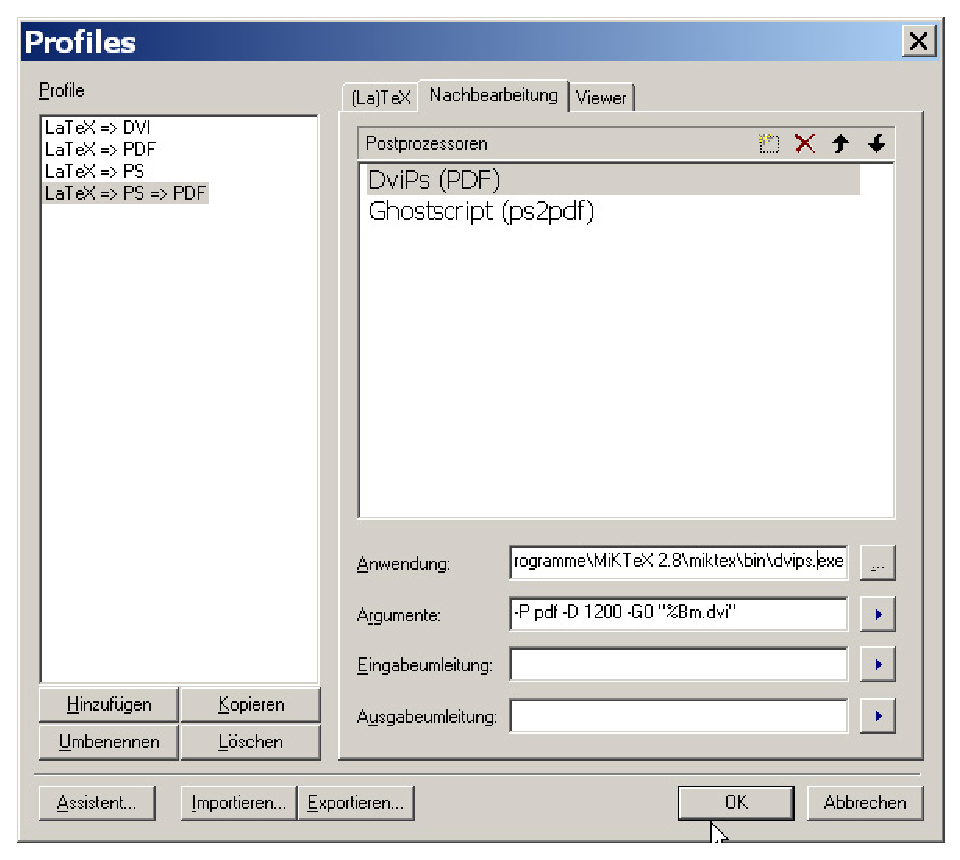
\includegraphics[scale=0.7]{./Bilder/latex2PS2PDF_Nachb_DviPs.eps}
  \caption{\label{fig_latex2ps2pdf_dvips}DviPS-Einstellungen f�r das Ausgabeprofil {\tt Latex => PS => PDF} }
\end{figure}
	%
	%
\begin{figure}%[hbt]
  \hfil 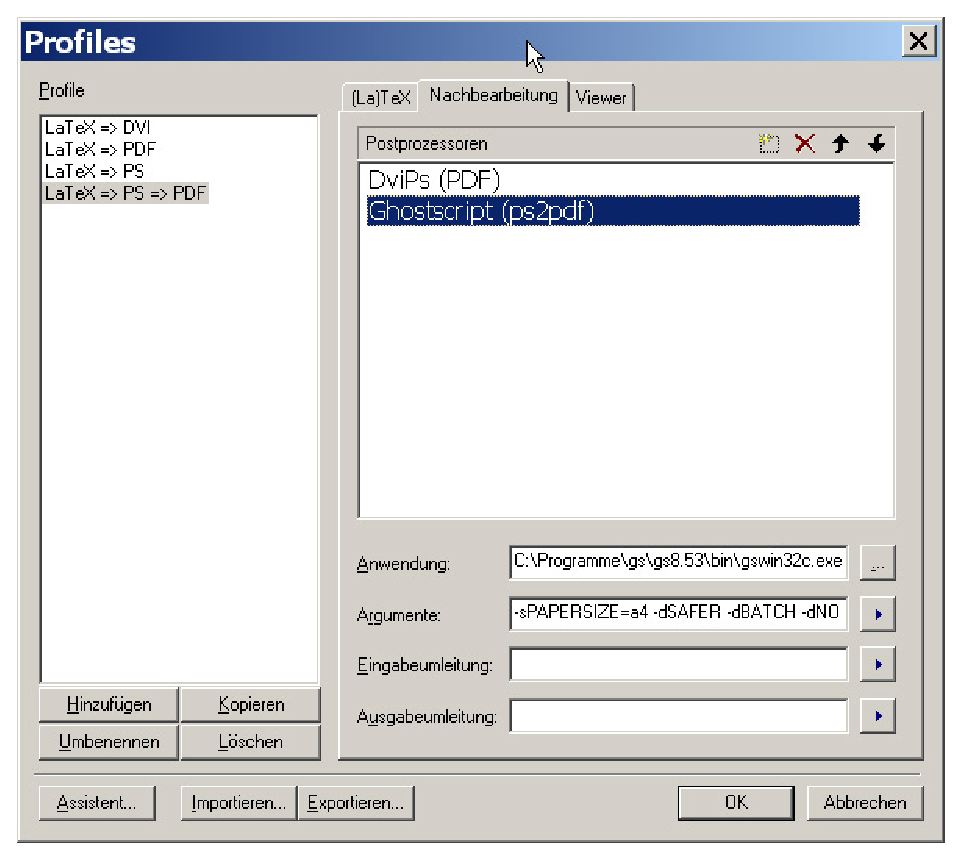
\includegraphics[scale=0.7]{./Bilder/latex2PS2PDF_Nachb_Ghost.eps}
  \caption{\label{fig_latex2dvi_ghost}GhostScript-Einstellungen f�r das Ausgabeprofil {\tt Latex => PS => PDF} }
\end{figure}
	%
Da die Parameter f�r GhostScript nicht vollst�ndig in der Abbildung zu sehen sind, hier die komplette Liste:
\begin{quote}
  {\tt -sPAPERSIZE=a4 -dSAFER -dBATCH -dNOPAUSE -sDEVICE=pdfwrite \\
       -dPDFSETTINGS=/prepress -dMaxSubsetPct=100 -dSubsetFonts=true\\
       -dEmbedAllFonts=true -sOutputFile=\grqq\%bm.pdf\grqq\ -c save pop -f\grqq\%bm.ps\grqq} 
 \end{quote}
	
	
Als Betrachter wird zum Beispiel der Acrobat Reader eingesetzt (\Abb{fig_latex2ps2pdf_viewer}).
	%
\begin{figure}%[hbt]
  \hfil \includegraphics[scale=0.7]{./Bilder/latex2PS2PDF_viewer.eps}
  \caption{\label{fig_latex2ps2pdf_viewer}Viewer-Einstellungen f�r das Ausgabeprofil {\tt Latex => PS => PDF} }
\end{figure}
	%

Der gro�e Vorteil von EPS f�r Diagramme etc. kehrt sich leider um f�r Rastergrafiken. Formate wie *.png oder *.tiff oder �hnliches werden nicht unterst�tzt. Die hier im Text gezeigten Screenshots wurden mit Photoshop ins EPS-Format konvertiert. Man kann auch zum Beispiel GIMP (www.gimp.org) zum Konvertieren nutzen. 

%--------------------------------------------------------------
\section{Hinweise zum \LaTeX-Befehlssatz}
%
%--------------------------------------------------------------
\subsection{Formatierung}
	%
Bei \LaTeX ist ``Times New Roman bereits die Standardeinstellung. Die Schriftgr��e, das Papierformat, die Sprache und die doppelseitige Formatierung werden zu Beginn des Dokumentes mit	\verb+\documentclass[12pt,a4paper,ngerman,twoside]{report}+ festgelegt. Die Angabe der Sprache ist wichtig f�r die automatische Silbentrennung, welche bei \LaTeX standardm��ig aktiviert ist. Probleme gibt es damit, wenn W�rter mit Umlauten am Ende einer Zeile stehen. Dann ben�tigt \LaTeX einen Trennvorschlag (z.B. \verb+Gesamt\-�ber\-sicht+), ansonsten wird das Wort nicht getrennt und auf den Seitenrand geschrieben.  
Der Zeilenabstand ist in diesem Dokument auf 1.1 gesetzt mit 
 (\verb+\renewcommand{\baselinestretch}{1.1}+).

%--------------------------------------------------------------
\subsection{Einbinden von Tabellen und Abbildungen}
	%
Das vorzeichensymmetrische Quantisieren wird durch die Schwellen $\pm{}T1$, $\pm{}T2$, $\pm{}T3$ festgelegt, welche
f{\"u}r alle Differenzen gelten. \Tabe{tab_thresholds} zeigt entsprechende Beispiele.
	%
\begin{table}
\centering % Zentrieren der Tabelle
  \caption{\label{tab_thresholds}Beispiel f�r das Einbinden von Tabellen}
\begin{tabular}{|c|c|c|c|}
  \hline
  Bereich & $Q_i$ & Bereich & $Q_i$\\
  \hline
  $\infty$ .. -T3 & -4 & T3 .. $\infty$ &4 \\
  -T3+1 .. -T2    & -3 & T2 .. T3-1     &3 \\
  -T2+1 .. -T1    & -2 & T1 .. T2-1     &2 \\
  -T1+1 .. -1     & -1 &  1 .. T1-1     &1 \\
  0               &  0 &                & \\
  \hline
\end{tabular}
\end{table}
	%
	
Abbildungen werden von \LaTeX\ automatisch entweder am oberen oder unteren Rand der Seite platziert. Die Referenz auf ein Bild muss gesetzt werden bevor das Bild eingebettet wird (siehe \Abb{fig_template}).
	%
\begin{figure}%[hbt]
  \hfil 
\includegraphics{template.eps}
  \caption{\label{fig_template}Beispiel f�r das Einbinden von Bildern}
\end{figure}
	%
Dadurch ist garantiert, dass das Bild in der N�he der Referenz erscheint, und fr�hestens auf derselben Seite wie die Referenz.
	%
%-------------------------------------------------
%
\subsection{Einbinden von Formeln}
%-------------------------------------------
	%
Dies ist eine Formel mit mehreren Zeilen, die am Gleichheitszeichen ausgerichtet sind
	%
\begin{align}\label{eq_abc}
	CX' &= 9 \cdot (9 \cdot Q1+Q2)+Q3 \\
	CX  &= |CX'| \nonumber\\ 
	SIGN &= sgn(CX') \;.
\end{align}
	%
Man beachte, dass die zweite Zeile keine Gleichungsnummer hat. Das Platzieren von Labels $\backslash${\tt label}\{{\tt xuz}\} erm�glicht auch Verweise auf Formeln, wie z.B.\ Gleichung (\ref{eq_abc}).  Es ist auch m�glich, mit {\tt$\backslash$begin}\{{\tt align*}\} f�r alle Zeilen das Nummerieren zu unterbinden:
	%
\begin{align*}\label{EQ_PREDERR}
\varepsilon = \left\{
		\begin{array}{lll}
		\hat{x} - x &:& SIGN < 0 \\
		x - \hat{x} &:& SIGN \geq 0
		\end{array}
	\right.
	\;.
\end{align*}
	%
Wenn eine Formel am Satzende steht, dann darf der Satzpunkt hinter der Formel nicht vergessen werden.
%-------------------------------------------------
%
\section{Literaturverzeichnis}
	%
Dieses Stylefile unterscheidet nicht zwischen Literatur- und Quellenverzeichnis.
Zum Referenzieren von Literatur wird ein System vorgeschlagen, dass die ersten drei Buchstaben des Nachnamens des Erstautors und die beiden letzten Ziffern des Jahres der Ver�ffentlichung enthalten \cite{Fli93}. Der Verweis erfolgte in diesem Fall mit \verb+\cite{Fli93}+. Die Literatureintr�ge sind dann alphabetisch zu sortieren. 
%Alternative ist auch ein Nummerieren in der Reihenfolge der Referenzierungen m�glich. Die erste Variante hat den Vorteil, dass der Leser aus der Angabe schon nach einmaligem Nachschlagen ableiten kann, um welche Literaturangabe es sich handelt. 


	
%-------------------------------------------------
\chapter{Kriterien zur Bewertung von Abschlussarbeiten}
\label{app_kriterien}
%----------------------------------------------
	%
Im Folgenden sind einzelne Punkte aufgelistet, die zur Bewertung einer Abschlussarbeit heran gezogen werden k�nnten.

%-------------------------------------------------
\section{Bewertung der schriftlichen Arbeit}
%

\paragraph{Form}
\begin{closelist}
  \item Layout-Vorgaben wurden eingehalten
  \item Satzbau/Fehlerfreiheit/Ausdruck
	\item L�nge der Arbeit ist angemessen
	\item Vollst�ndige Tabellen und Grafiken (Tabellenk�pfe, Legenden)
	\item Grafiken sind textuell erl�utert
	\item Wissenschaftliche Ausdrucksweise
\end{closelist}

\paragraph{Aufbau und Inhalt}
\begin{closelist}
	\item Ausgewogene Gliederung
	\item Inhaltlich richtige Darstellung
	\item Eigenleistung erkennbar
 \item Bearbeitung zeigt, dass fundierte/aktuelle Kenntnisse in der Thematik erworben wurden
 \item Gestellte Aufgabe ist vollst�ndig gel�st/behandelt
	\item Alle Randbedingungen sind dargestellt
	\item Zielsetzung, Vorgehen und Bedeutung des Themas sind klar beschrieben
	\item Alle wichtigen Begriffe sind definiert, Grundlagen ausgewogen dargestellt
	\item Ergebnisse der Arbeit sind klar herausgearbeitet und interpretiert
	\item Entscheidungsfindung bei der Auswahl von Methoden oder Verfahrensweisen ist erkennbar
\end{closelist}

\paragraph{Zitierweise/Nachweisbarkeit}
\begin{closelist}
	\item Alle �bernahmen sind zitiert, alle Thesen/Behauptungen belegt
	\item Aktuelle Literatur / relevante Autoren
	\item Einheitliche Zitierweise
  \item Vollst�ndiges und richtiges Literaturverzeichnis
\end{closelist}
	%
%-------------------------------------------------
\section{Bewertung der Arbeitsweise und der Ergebnisse}
%
%-------------------------------------------------
\paragraph{Schwierigkeit der Aufgabenstellung}
%
\begin{closelist}
	\item Aufgabe ist komplex
	\item Neuland/keine Vorarbeiten waren vorhanden
\end{closelist}

\paragraph{Eigenst�ndigkeit}
\begin{closelist}
	\item ad�quate Literatur wurde eigenst�ndig recherchiert
	\item es wurde �berwiegend selbst�ndig ohne Korrekturen des Betreuers gearbeitet
	\item geeignete Methoden wurden selbst�ndig ausgew�hlt
  \item �ber alternative L�sungswege wurde nachgedacht
  \item Kontakte zur externen Personen wurden eigenst�ndig gekn�pft
	\item Kreativit�t/eigene Ideen wurden eingebracht
\end{closelist}

\paragraph{Resultat (Software, Demonstrator, Hardware)}
\begin{closelist}
	\item ist voll funktionst�chtig
	\item ist sauber ausgef�hrt (z.B. Kommentare bei Software)
	\item Abgegebene Unterlagen erm�glichen eine Reproduktion
 der Ergebnisse
\end{closelist}

\paragraph{Sonstiges}
\begin{closelist}
	\item wissenschaftliche Arbeitsweise erkennbar
	\item Hinweise des/der Betreuer wurden angenommen
	\item die erreichten Ergebnisse passen zur Aufgabenstellung
	\item Ergebnisse sind f�r weitere Arbeit der Arbeitsgruppe relevant
\end{closelist}

	
%-------------------------------------------------
\chapter{Information zur Abgabe von Abschlussarbeiten}
\label{app_abgabe}
%----------------------------------------------
	%

Gemeinsam mit der schriftlichen Arbeit ist eine CD-ROM abzugeben. Im Sinne der Prinzipien zur Sicherung der guten wissenschaftlichen Praxis muss diese CD alle Daten und Informationen enthalten, welche erforderlich sind, um die Ergebnisse der Arbeit zu reproduzieren. Es wird folgende Verzeichnisstruktur empfohlen:
\begin{itemize}
	\item Thesis
	\begin{itemize}
		\item Hier stehen alle Quellen (*.tex, *.sty, *.doc, *.txt), welche f�r das Anfertigen der schriftlichen Arbeit genutzt wurden.
		\item Au�erdem sind hier alle Bilder, welche in der Arbeit zu sehen sind, in einem geeigneten Format (EPS, oder hochaufgel�st) abgelegt.
		\item Hinweise, mit welchem Textverarbeitungssystem (inkl. Tools) die Arbeit geschrieben wurde
	\end{itemize}
	\item Testdaten
	\begin{itemize}
		\item alle Daten, welche f�r die Untersuchungen  verwendet wurden
	\end{itemize}
	\item Quellcode
	\begin{itemize}
		\item Quellcode, der zu Beginn der Arbeit zur Verf�gung stand
		\item externer Quellcode, der eingebunden wurde
		\item Quellcode des fertigen Programms / der fertigen Programme
	\end{itemize}
	\item Untersuchungen
	\begin{itemize}
		\item Ergebnisse: Listen (*.txt, *.xls, ...) mit den numerischen Ergebnissen der Untersuchungen
		\item Batchfiles (*.bat, Programmaufrufe mit entsprechenden Parametern und Optionen), mit denen die Ergebnisse erneut erzeugt werden k�nnen
		\item Typischer Weise gibt es hier entsprechend des Themas weitere Unterverzeichnisse.
	\end{itemize}
	\item Literatur
	\begin{itemize}
		\item alle Artikel und andere Quellen (*.pdf, *.doc, *.html, ...), welche w�hrend der Recherche gefunden und in der Arbeit zitiert wurden  
	\end{itemize}
\end{itemize}
Ferner muss die CD eine ReadMe.txt-Datei enthalten, welche Hinweise zum Inhalt gibt und auch den Inhalt von evtl. anderen Ordnern erl�utert. Au�erdem ist die Thesis als PDF-File im Wurzelverzeichnis abzulegen.
	%
% set the correct properties of final pdf file
% as the hyperref settings are overwritten by all *.eps files

\includegraphics{./authoring.eps}

	%
\end{document}
